\documentclass[dvipdfmx,a4paper,11pt]{jsarticle}


% 数式
\usepackage{amsmath,amsfonts}
\usepackage{bm}
\usepackage{amsthm}
\usepackage{amssymb}
\usepackage{tcolorbox}
% 画像
% \usepackage[dvipdfmx]{graphicx,color}

\usepackage[%
dvipdfmx, %欧文ではコメントアウトする
setpagesize=false,
bookmarks=true,
bookmarksdepth=tocdepth,
bookmarksnumbered=true,
colorlinks=true,
linkcolor=blue,
citecolor=blue,
urlcolor=blue,
pdftitle={},
pdfsubject={},
pdfauthor={},
pdfkeywords={}
]{hyperref}

\usepackage{pxjahyper}
\usepackage{tikz}
\usetikzlibrary{intersections,calc,arrows.meta}
\usepackage[truedimen,top=25truemm,bottom=30truemm,hmargin=25truemm]{geometry}
\usepackage{calc}


\begin{document}
\theoremstyle{plain}
\newtheorem{thm}{Theorem}[section]
\newtheorem{lem}[thm]{Lemma}
\newtheorem{prop}[thm]{Proposition}
\newtheorem{cor}[thm]{Corollary}
\newtheorem{conj}[thm]{Conjecture}

\theoremstyle{definition}
\newtheorem{ass}[thm]{Assumption}
\newtheorem{dfn}[thm]{Definition}

\theoremstyle{remark}
\newtheorem{rem}[thm]{Remark}

\theoremstyle{plain}
\newtheorem*{thm*}{Theorem}
\newtheorem*{lem*}{Lemma}
\newtheorem*{prop*}{Proposition}
\newtheorem*{cor*}{Corollary}
\newtheorem*{conj*}{Conjecture}

\theoremstyle{definition}
\newtheorem*{ass*}{Assumption}
\newtheorem*{dfn*}{Definition}

\theoremstyle{remark}
\newtheorem*{Proof}{Proof}

\numberwithin{equation}{section}

\theoremstyle{remark}
\newtheorem*{rem*}{Remark}

% \setlength{\topmargin}{-20truemm}
% \setlength{\headheight}{0pt}
% \setlength{\headsep}{0pt}
\setlength{\footskip}{20truemm}


% \setlength{\@tempdima}{1pt*\ratio{\dimexpr\textheight/\@lines}{\baselineskip}}
% \renewcommand{\baselinestretch}{\strip@pt\@tempdima}\selectfont

\makeatletter
\newcount\@chars\newcount\@lines
\@chars=40                      % 1行の文字数
\@lines=40                      % 1ページの行数

\newdimen\@kanjiskip
\@kanjiskip=\dimexpr(\textwidth-1zw*\@chars)/\numexpr\@chars-1
\newdimen\@@kanjiskip
\@@kanjiskip=\dimexpr\@kanjiskip/10

\baselineskip=\dimexpr\textheight/\@lines
\kanjiskip=\@kanjiskip plus \@@kanjiskip minus \@@kanjiskip
\parindent=\dimexpr 1zw+2truept
\parindent=\dimexpr\parindent+\@kanjiskip
\makeatother

% ↑は貼り付けただけなのでわからない。

\title{位相幾何}
\date{}
\author{Fefr}
\maketitle
\tableofcontents
\clearpage

%--------------------本文--------------------%

\section{位相空間の(コ)ホモロジー}

\subsection{圏と関手}

圏の定義は略。\\
圏の例をすこしあげる。
\begin{tcolorbox}[title = 例1]
  位相空間$X$から位相空間$Y$への写像の族$f_{t}:X\to Y$に対し、写像$F:X\times [0,1] \to Y$を
  \begin{equation*}
    F(x,t)=f_{t}(x)\qquad (x\in X,t \in [0,1])
  \end{equation*}
  で定義するとき、$F$が連続ならば写像族$\{f_t\}$を$f_0$から$f_1$への\textgt{ホモトピー}(homotopy)という。\\
  連続写像$f,f':X\to Y$に対し、$f$から$f'$へのホモトピーが存在するとき$f$は$f'$に\textgt{ホモトープ}(homotop)
  であるといい、$f\simeq f':X\to Y$で表す。\\
  ホモトープという関係は同値関係となる。\\
  実際、反射律は$f\simeq f:X\to Y$は$f_{t}=f$とすることにより、対称律は$f\simeq f':X\to Y$とすると、
  $f'$の$f$へのホモトピー$\{f'_{t}\}$は$f$の$f'$へのホモトピー$\{f_{t}\}$を用いて$f'_{t}=f_{1-t}$で与えられる。
  推移律は、$f\simeq f',f'\simeq f'':X\to Y$ならば$f$の$f''$へのホモトピー$\{h_{t}\}$が
  $f$から$f'$へのホモトピー$\{f_{t}\}$、$f'$から$f''$へのホモトピー$\{g_{t}\}$を用いて
  \begin{equation*}
    h_{t}=\left\{ 
    \begin{alignedat}{2}   
      &f_{2t}  \quad &(0\leq t\leq 1/2)\\   
      &g_{2t-1}\quad &(1/2\leq t\leq 1)
    \end{alignedat} 
    \right.
  \end{equation*}
  で与えられる。\\
  上の同値類を連続写像の\textgt{ホモトピー類}(homotopy class)という。\\
  明らかに$f\simeq f':X\to Y$で$g\simeq g':Y\to Z$ならば\\
  \begin{equation*}
    g\circ f\simeq g\circ f'\simeq g'\circ f'\simeq g'\circ f:X \to Z
  \end{equation*}
  である。($\{g\circ f_{t}\}$が$g\circ f$から$g\circ f'$へのホモトピーを与え、$\{g_{t}\circ f'\}$が$g\circ f'$から$g'\circ f'$へのホモトピーを与える。)\\
  すなわち、ホモトープな連続写像の合成はホモトープである。\\
  よって、対象を位相空間とし、射を連続写像のホモトピー類で定義することにより、1つの圏が得られる。
\end{tcolorbox}

\clearpage

\begin{tcolorbox}[title = ホモトープな例,colbacktitle = lime!80!black]
  $X=\mathbf{R},Y=\mathbf{R}^2$とし、それぞれ通常の位相を入れる。そして、$f,g:X\to Y$を
  \begin{equation*}
    f(x)=(x,0),\qquad g(x)=(x,1)
  \end{equation*}
  で定義する。そして、$F:X\times [0,1]\to Y$を
  \begin{equation*}
    F(x,t)=(x,t)
  \end{equation*}
  で定義すれば、$F(x,0)=f(x),F(x,1)=g(x)$となり、位相空間論の知識より$F,f,g$は連続なので$f,g$はホモトープである。
\end{tcolorbox}

加群,加群の準同型写像の定義は略。$R$加群、$R$準同型写像を単に加群、準同型写像という。
簡単のため$R$を可換環と仮定する。可換性が必要がない場面もある。
\begin{tcolorbox}[title = 例2]
  整数の集合$\mathbf{Z}$を添字集合とする$R$上の加群の族$C=\{C_{q}\}$を$R$上の\textgt{次数つき加群}(graded module)
  といい、$C_{q}$の元$c$を$C$の\textgt{次数$q$の元}といって、$q=\text{deg}\ c$と書く。$C,C'$を次数つき加群とし、
  $d$を1つの整数とする。このとき$\mathbf{Z}$を添字集合とする準同型写像$\varphi_{q}:C_{q} \to C_{q+d}$の族$\varphi = \{\varphi_{q}\}$を
  $C$から$C'$への\textgt{次数$d$の準同型写像}といい、$\varphi : C\to C'$で表す。\\
  $C''$も加群とし、$\varphi' : C'\to C''$を次数$d'$の準同型写像とするとき、次数$d+d'$の準同型写像$\varphi' \circ \varphi : C\to C''$を
  \begin{equation*}
    (\varphi' \circ \varphi)_{q} = \varphi'_{d+q} \circ \varphi_{q}
  \end{equation*} 
  で定義し、$\varphi$と$\varphi'$の合成という。
  いま、次の二つの圏が得られる。
  \begin{itemize}
    \item 次数つき加群を対象とし、任意の次数の準同型写像を射とする圏
    \item 次数つき加群を対象とし、次数$0$の準同型写像を射とする圏
  \end{itemize}
\end{tcolorbox}

\begin{tcolorbox}[title = 例3]
  $R$上の次数つき加群$C$において、次数$-1$の準同型写像$\partial : C\to C$で
  \begin{equation*}
    \partial \circ \partial = 0
  \end{equation*}
  を満たすものが与えられたとき、$(C,\partial)$を\textgt{$R$上のチェイン複体}(chain complex)という。
  チェイン複体は加群$C_{q}$と準同型写像$\partial_{q}:C_{q}\to C_{q-1}$の列
  \begin{center}
    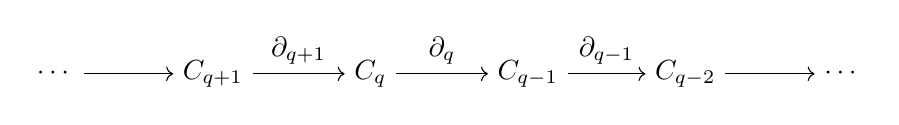
\begin{tikzpicture}[auto]
      \node (a) at (0, 1.2) {$\cdots$}; \node (b) at (2.0, 1.2) {$C_{q+1}$};
      \node (c) at (4.0, 1.2) {$C_{q}$}; \node (d) at (6.0, 1.2) {$C_{q-1}$};
      \node (e) at (8.0, 1.2) {$C_{q-2}$}; \node (f) at (10.0, 1.2) {$\cdots$};
      
      \draw[->] (a) to node {} (b); \draw[->] (b) to node {$\partial_{q+1}$} (c);
      \draw[->] (c) to node {$\partial_{q}$} (d); \draw[->] (d) to node {$\partial_{q-1}$} (e);
      \draw[->] (e) to node {} (f);
    \end{tikzpicture}
  \end{center}
  で、各$q$に対し
  \begin{equation*}
    \partial_{q-1} \circ \partial_{q} = 0
  \end{equation*}
  の成り立つもの、と言い換えることができる。$\partial = \{\partial_{q}\}$を\textgt{バウンダリ作用素}(boundary operator)という。
  チェイン複体$(C,\partial)$を単に$C$で表す。\\
  $C,C'$をチェイン複体とするとき、次数$0$の準同型写像$\varphi : C\to C'$で、$C,C'$のバウンダリ作用素$\partial,\partial'$に対し
  \begin{equation*}
    \partial' \circ \varphi = \varphi \circ \partial
  \end{equation*}
  を満たすものを\textgt{チェイン写像}(chain map)という。すなわち、準同型写像$\varphi_{q} : C_{q} \to C'_{q}$の族
  $\varphi = \{\varphi_{q}\}$で、各$q$に対し
  \begin{equation*}
    \partial_{q}' \circ \varphi_{q} = \varphi_{q-1} \circ \partial_{q}
  \end{equation*}
  の成り立つものがチェイン写像である。\\
  チェイン複体の恒等写像(恒等射)はチェイン写像であり($\partial'\varphi = \varphi\partial$で次数$0$だから)\\
  チェイン写像の合成はチェイン写像である。(確かめること)\\
  よって、チェイン複体を対象とし、射をチェイン写像とすることにより、1つの圏を得る。
\end{tcolorbox}

\begin{tcolorbox}[title = 例4]
  チェイン写像$\varphi,\varphi':C\to C'$に対し、次数$+1$の準同型写像$\Phi : C\to C'$があって、
  \begin{equation*}
    \partial' \circ \Phi + \Phi \circ \partial = \varphi - \varphi'
  \end{equation*}
  が成り立つとき、$\varphi$は$\varphi'$への\textgt{チェインホモトープ}(chain homotopic)であるといい、$\varphi \simeq \varphi' : C\to C'$で表す。
  $\Phi$を$\varphi$の$\varphi'$への\textgt{チェインホモトピー}(chain homotopy)という。\\
  チェインホモトープという関係は$C$から$C'$へのチェイン写像の集合における同値関係である。
  この同値類を\textgt{チェインホモトピー類}(chain homotopy class)という。\\
  反射律は$\Phi=0$とすれば$\varphi \simeq \varphi : C\to C'$がわかる。対称律は$\varphi \simeq \varphi' : C\to C'$のチェインホモトピーを$\Phi$とすると、
  $\Phi'=-\Phi$と置くことにより$\Phi'$は$\varphi'$から$\varphi$へのチェインホモトピーとなる。\\
  $\varphi\simeq \varphi' : C\to C'$で$\psi \simeq \psi' :C' \to C''$ならば、$\psi \circ \varphi \simeq \psi' \circ \varphi' : C\to C''$
  である。実際、$\Phi$を$\varphi$から$\varphi'$への、$\Psi$を$\psi$から$\psi'$へのチェインホモトピーとするとき
  \begin{equation*}
    \psi'\circ \Phi + \Psi \circ \varphi : C\to C''
  \end{equation*}
  は$\psi \circ \varphi$から$\psi'\circ \varphi'$へのチェインホモトピーである。\\
  よって、チェイン複体を対象とし、チェイン写像のチェインホモトピー類を射とすることにより、1つの圏が得られる。
\end{tcolorbox}
同型射、同型、関手の定義は略。例1の圏における同型射、同型はふつう\textgt{ホモトピー同値写像}(homotopy equivalent map?)、\textgt{ホモトピー同値}(homotopy equivalent)とよばれている。\\
例4での同型射を\textgt{チェイン同値写像}(chain equivalent map?)という。
\begin{tcolorbox}[title = 例5]
  $C$をチェイン複体とする。
  \begin{equation*}
    Z_{q}(C)=\text{Ker}\, \partial_{q},\qquad B_{q}(C)=\text{Im}\, \partial_{q+1}
  \end{equation*}
  とおけば、$\partial_{q}\circ \partial_{q+1} = 0$だから、$B_{q}(C)\subset Z_{q}(C)$である。商加群
  \begin{equation*}
    H_{q}(C)=Z_{q}(C)/B_{q}(C)
  \end{equation*}
  を$C$の\textgt{$q$ホモロジー群}(q-homology group?)といい、次数つき加群$H_{*}(C)=\{H_{q}(C)\}$を$C$の\textgt{ホモロジー群}(homology groups)という。
  $C_q$の元を$C$の\textgt{$q$チェイン}(q-chain?)。$Z_{q}(C)$の元を\textgt{$q$サイクル}(q-cycle?)(。$B_{q}(C)$の元を\textgt{$q$バウンダリ}(q-boundary?)といい、
  $c\in Z_{q}(C)$で代表される$H_{q}(C)$の元を$[c]$で表して、$c$の\textgt{ホモロジー類}(homology class)という。\\
  チェイン写像$\varphi : C\to C'$は$C$の$q$サイクル、$q$バウンダリを$C'$の$q$サイクル、$q$バウンダリに移す。
  実際、$c\in Z_{q}(C)=\text{Ker}\, \partial_{q}$をとると、$\partial_{q}(c)=0$だから
  \begin{equation*}
    \partial_{q}'(\varphi(c))=(\partial'_{q} \circ \varphi)(c)=(\varphi \circ \partial_{q})(c)=\varphi(\partial_{q}(c))=\varphi(0)=0
  \end{equation*}
  よって、$c\in Z_{q}(C)\Rightarrow \varphi(c)\in Z_{q}(C')$が成り立つ。\\
  また、$a\in B_{q}(C)$をとると、ある$b\in C_{q+1}$があって$a=\partial_{q+1}(b)$を満たすから
  \begin{equation*}
    \varphi(a)=\varphi(\partial_{q+1}(b))=(\varphi \circ \partial_{q+1})(b)=(\partial'_{q+1} \circ \varphi)(b)=\partial'_{q+1}(\varphi(b))\in B_{q}(C')
  \end{equation*}
  よって、$c\in B_{q}(C)\Rightarrow \varphi(c)\in B_{q}(C')$が成り立つ。\\
  したがって次数$0$の準同型写像$H_{*}(\varphi) : H_{*}(C)\to H_{*}(C')$が
  \begin{equation*}
    H_{*}(\varphi)([c])=[\varphi(c)]\qquad (c\in Z_{q}(C))
  \end{equation*}
  により定義される。$H_{*}(\varphi)$を$\varphi$により\textgt{誘導される準同型写像}(induced homomorphism?)といい、しばしば$\varphi_{*}$でかく。
  明らかに、$H_{*}(1)=1,H_{*}(\varphi \circ \varphi')=H_{*}(\varphi)\circ H_{*}(\varphi')$である。
  したがって$H_{*}$はチェイン複体とチェイン写像の圏(例3)から次数つき加群と次数$0$の準同型写像の圏(例2(2))への共変関手である。
  $H_{*}$を\textgt{ホモロジー函手}(homology functor)という。
\end{tcolorbox}
\begin{tcolorbox}[title = 例6]
  チェイン写像$\varphi,\varphi' : C\to C'$がチェインホモトープならば、$\varphi$の$\varphi'$へのチェインホモトピー$\Phi$に対し
  \begin{equation*}
    \varphi(c)-\varphi'(c)=\partial(\Phi(c))\qquad (c\in Z_{q}(C))
  \end{equation*}
  だから、$[\varphi(c)]=[\varphi'(c)]$で、したがって、$H_{*}(\varphi)=H_{*}(\varphi'):H_{*}(C)\to H_{*}(C')$
  よってホモロジー函手$H_{*}$はまたチェイン複体とチェイン写像のチェインホモトピー類の圏(例4)から次数つき加群と次数$0$の準同型写像の圏への共変函手ともみられる。
\end{tcolorbox}

\begin{tcolorbox}[title = 例7]
  位相空間$X$に対し、$X$の弧状連結成分の集合を考え、これより生成される自由加群を$H_{0}(X)$で表す。
  また、位相空間の間の連続写像$f:X\to Y$に対し、次の条件によって準同型写像$H_{0}(f):H_{0}(X)\to H_{0}(Y)$
  を定義する。$X$の弧状連結成分$X_{\lambda}$に対し、$H_{0}(f)(X_{\lambda})$は$f(X_{\lambda})$を含む$Y$の弧状連結成分を表す。
  明らかに連続写像$f,g:X\to Y$がホモトープならば$H_{0}(f)=H_{0}(g)$\\
  $H_{0}$は位相空間と連続写像の圏、または位相空間と連続写像のホモトピー類の圏(例1)から加群の圏への共変函手である。
\end{tcolorbox}
また、函手の定義から函手は同型を保存することがわかる。

\clearpage

\subsection{特異ホモロジー}
$q$次元Euclid空間を$\mathbf{R}^q$で表し、その原点を$P_0$,第$i$軸上の単位点を$P_i$で表す($i=1, \cdots ,q$).\ 
$P_{0},P_{1},\cdots,P_{q}$で張られる$q$次元単体を$\Delta^q$で表し、\textgt{標準$q$単体}(standard q-simplex)という。$\Delta^1=[0,1]$である。
%---------q単体の図をかく---------%




%--------------------------------%
$q\geq 1$と$i=0,1,\cdots,q$に対し、
\begin{equation*}
  \varepsilon^{i}_{q}:\Delta^{q-1}\to \Delta^{q}
\end{equation*}
によって
\begin{equation*}
  \varepsilon^{i}_{q}(P_{j})=\left\{
    \begin{alignedat}{2}
      &P_{j}\quad &(j<i)\\
      &P_{j+1}\quad &(j\geq i)
    \end{alignedat}
  \right.
\end{equation*}
なる線型写像を表す。場合分けにより容易に確認できるが次が成り立つ。
\begin{equation}
  \varepsilon^{j}_{q+1} \circ \varepsilon^{i}_{q}=\varepsilon^{i}_{q+1}\circ \varepsilon^{j-1}_{q}\quad (i<j)
\end{equation}
位相空間$X$が与えられたとき、任意の連続写像$\sigma : \Delta^{q}\to X$を$X$の\textgt{特異$q$単体}(singular q-simplex)という($q\geq 0$).\ 
$q>0$のとき、各$i=0,1,\cdots,q$に対し、特異$q-1$単体$\sigma \circ \varepsilon^{i}_{q} : \Delta^{q-1}\to X$が得られるが、
これを$d_{i}\sigma$で表し、$\sigma$の\textgt{第$i$面}(i-face?)という。\\
いま、単位元$1$をもつ可換環$R$が与えられたとする。このとき次数つき加群$S(X)=\{S_{q}(X)\}$を$q\geq 0$ならば
$S_{q}(X)$は$X$のすべての特異$q$単体の集合によって生成される自由加群を表し、$q<0$ならば$S_{q}(X)=0$であるとして
定義する。さらに次数$-1$の準同型写像$\partial : S(X)\to S(X)$を
\begin{equation*}
  \partial_{q}=\left\{
  \begin{alignedat}{2}
    &\sum_{i=0}^{q}(-1)^{i}d_{i}\quad &(q>0)\\
    &0 \quad &(q\leq 0)
  \end{alignedat}
  \right.
\end{equation*}
によって定義する。ここに$d_{i}:S_{q}(X)\to S_{q-1}(X)$は$\sigma$を$d_{i}\sigma$にうつす準同型写像(これを\textgt{面作用素}(英訳がわからない)という)\\
(1.1)より明らかに
\begin{equation}
  d_{i}\circ d_{j}=d_{j-1}\circ d_{i}\quad (i<j)
\end{equation}
したがって
\begin{align*}
  \partial_{q}\circ \partial_{q+1}
  &=\sum_{i,j}(-1)^{i+j}d_{i}\circ d_{j}\\
  &=\sum_{i<j}(-1)^{i+j}d_{i}\circ d_{j} + \sum_{i\geq j}(-1)^{i+j}d_{i}\circ d_{j}\\
  &=\sum_{i<j}(-1)^{i+j}d_{j-1}\circ d_{i} + \sum_{i\geq j}d_{i}\circ d_{j}\\
  &=\sum_{i\leq j}(-1)^{i+j+1}d_{j}\circ d_{i} + \sum_{i\leq j}(-1)^{i+j}d_{j}\circ d_{i}\\
  &=0
\end{align*}
よって$S(X)$は$\partial$をバウンダリ作用素としてチェイン複体である。\\
これを(Rに係数をもつ)\textgt{$X$の特異チェイン複体}(singular chain complex)という。\\
$f:X\to Y$を位相空間の間の連続写像とする。このとき$X$の任意の特異$q$単体$\sigma : \Delta^q \to X$
に対し、合成$f\circ \sigma : \Delta^q \to Y$は$Y$の特異$q$単体である。明らかに
\begin{equation*}
  d_{i}(f\circ \sigma)=f\circ (d_{i}\sigma)
\end{equation*}
したがってチェイン写像$S(f):S(X)\to S(Y)$が$\sigma$を$f\circ \sigma$にうつすことによって定義される。
$S$は位相空間と連続写像の圏からチェイン複体とチェイン写像の圏への共変函手であることが容易に示される。$S$を\textgt{特異チェイン函手}という。\\
なお、$S(f)$をしばしば$f_{\sharp}$で表す。\\
特異チェイン複体$S(X)$のホモロジー群$H_{*}(S(X))=\{H_{q}(S(X))\}$を$H_{*}(X)=\{H_{q}(X)\}$で表し、位相空間$X$の\textgt{(特異)ホモロジー群}という。また、
連続写像$f:X\to Y$に対し、チェイン写像$S(f)$より誘導される準同型写像$S(f)_{*}:H_{*}(X)\to H_{*}(Y)$を$f_{*}$で表し、
$f$より\textgt{誘導される準同型写像}という。\\
基礎環$R$を明示するときは、$H_{*}(X)$は$H_{*}(X;R)$と書かれ、$R$に\textgt{係数をもつホモロジー群}とよばれる。\\
いま、位相空間と連続写像の圏から次数つき加群と次数$0$の準同型写像の圏への共変函手が位相空間$X$に$H_{*}(X)$を、
連続写像$f:X\to Y$に$f_{*}:H_{*}(X)\to H_{*}(Y)$を対応されることにより得られるが、これを\textgt{特異ホモロジー函手}という。\\
定義より明らかに
\begin{equation*}
  H_{q}(X)=0\quad (q<0)
\end{equation*}
$H_{0}(X)$を考えよう。特異$0$単体$\sigma : \Delta^{0}\to X$はその像$\sigma(\Delta^{0})$によって定まる。
したがって$X$の特異$0$単体は$X$の点と同一視してよい。定義より明らかに、すべての特異$0$単体はサイクルであり、これらの$2$つ$x,x'\in X$は同一の弧状連結成分に
属しているときしかもそのときに限り同一のホモロジー類を代表する。したがって$0$ホモロジー群$H_{0}(X)$は$X$の弧状連結成分の集合によって生成される自由加群である。
さらに、連続写像$f:X\to Y$に対し$S(f)(x)=f(x)\ (x\in X)$だから、$f_{*}:H_{0}(X)\to H_{0}(Y)$は$X$の弧状連結成分$X_{\lambda}$を$f(X_{\lambda})$を含む$Y$の弧状連結成分にうつす。\\

\begin{tcolorbox}[title = 補題1,upperbox = visible]
  $X$を位相空間とし、$i_{0},i_{1}:X\to X\times [0,1]$を
  \begin{equation*}
    i_{0}(x)=(x,0),\quad i_{1}(x)=(x,1)\quad (x\in X)
  \end{equation*}
  で与えられる連続写像とする。このときチェイン写像$i_{0\sharp},i_{1\sharp}:S(X)\to S(X\times [0,1])$はチェインホモトープである。
  \tcblower
  \textgt{証明}\\
  各$q\geq 0$と各$i=0,1,\cdots,q$に対し、
  \begin{equation*}
    \theta_{q+1}^{\, i}:\Delta^{q+1}\to \Delta^{q}\times [0,1]
  \end{equation*}
  によって
  \begin{equation*}
    \theta_{q+1}^{\, i}(P_{j})=\left\{
      \begin{alignedat}{2}
        &(P_{j},0)\quad &(j\leq i)\\
        &(P_{j-1},1)\quad &(j>i)
      \end{alignedat}
    \right.
  \end{equation*}
  なる線型写像を表す。\\
  $X$の各特異$q$単体$\sigma : \Delta^{q}\to X$に対し、$X\times [0,1]$の特異$q+1$単体
  \begin{center}
    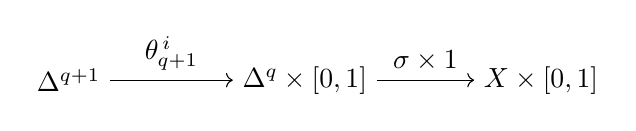
\begin{tikzpicture}[auto]
      \node (a) at (0,1.2) {$\Delta^{q+1}$}; \node (b) at (3.0,1.2) {$\Delta^{q}\times [0,1]$}; \node (c) at (6.0,1.2) {$X\times [0,1]$};
      
      \draw[->] (a) to node {$\theta_{q+1}^{\, i}$} (b); \draw[->] (b) to node {$\sigma \times 1$} (c);
    \end{tikzpicture}
  \end{center}
  を$D_{i}\sigma$で表し、準同型写像$D_{i}: S_{q}(X)\to S_{q+1}(X\times [0,1])$は$\sigma$を$D_{i}\sigma$にうつすものと定義しよう。容易に
  \begin{align}
    \begin{alignedat}{2}
      &d_{0}\circ D_{0}=i_{1\sharp},\quad d_{q+1}\circ D_{q}=i_{0\sharp},\quad d_{i}\circ D_{i}=d_{i}\circ D_{i-1}\\
      &d_{i}\circ D_{j}=D_{j-1}\circ d_{i}\quad (j>i),\quad d_{i}\circ D_{j}=D_{j}\circ d_{i-1}\quad (j+1<i) 
    \end{alignedat}
  \end{align}
  が成り立つことがわかる。\\
  いま、次数$+1$の準同型写像$\Phi : S(X)\to S(X\times [0,1])$を
  \begin{equation*}
    \Phi_{q}=\sum_{i=0}^{q}(-1)^{i}D_{i}
  \end{equation*}
  によって定義すれば、(1.3)より$\Phi$は$i_{1\sharp}$から$i_{0\sharp}$へのチェインホモトピーであることがわかる。実際、
  \begin{align*}
    \partial_{q+1}\circ \Phi_{q}
    &=\sum_{i,j}(-1)^{i+j}d_{i}\circ D_{j}\\
    &=(\sum_{i<j}(-1)^{i+j}d_{i}\circ D_{j})+(\sum_{i}d_{i}\circ D_{i}-\sum_{i}d_{i}\circ D_{i-1})+(\sum_{i>j+1}(-1)^{i+j}d_{i}\circ D_{j})\\
    &=(\sum_{i<j}(-1)^{i+j}D_{j-1}\circ d_{i})+(d_{0}\circ D_{0}-d_{q+1}\circ D_{q})+(\sum_{i>j+1}(-1)^{i+j}D_{j}\circ d_{i-1})\\
    &=(\sum_{i\leq j}(-1)^{i+j+1}D_{j}\circ d_{i})+(i_{1\sharp}-i_{0\sharp})+(\sum_{i>j}(-1)^{i+j+1}D_{j}\circ d_{i})\\
    &=\sum_{i,j}(-1)^{i+j+1}D_{j}\circ d_{i}+(i_{1\sharp}-i_{0\sharp})\\
    &=-\Phi_{q-1}\circ \partial_{q}+(i_{1\sharp}-i_{0\sharp})
  \end{align*}
\end{tcolorbox}

\clearpage

\begin{tcolorbox}[title = 定理1,upperbox = visible]
  $X,Y$を位相空間とし、$f_{0},f_{1}:X\to Y$をホモトープな連続写像とする。このときチェイン写像$f_{0\sharp},f_{1\sharp}:S(X)\to S(Y)$はチェインホモトープで、したがって
  \begin{equation*}
    f_{0*}=f_{1*}:H_{*}(X)\to H_{*}(Y)
  \end{equation*}
  \tcblower
  \textgt{証明}\\
  $F:X\times [0,1]\to Y$を$f_{0}$から$f_{1}$へのホモトピーとする。上の補題の
  $i_{0},i_{1}:X\to X\times [0,1]$に対し、$F\circ i_{0}=f_{0},\ F\circ i_{1}=f_{1}$
  が成り立つ。したがって補題1により
  \begin{equation*}
    f_{0\sharp}=F_{\sharp}\circ i_{0\sharp}\simeq F_{\sharp}\circ i_{1\sharp}=f_{1\sharp}
  \end{equation*}
\end{tcolorbox}
$C,C'$は次数つき加群で、各$q$に対し$C'_{q}$は$C_{q}$の部分加群のとき、$C'$を次数つき加群$C$の\textgt{部分加群}という。$C'$がチェイン複体で、さらに各$q$に対し$\partial_{q}(C'_{q})\subset C'_{q-1}$が成り立つならば、$C'$をチェイン複体$C$の\textgt{部分複体}という。
部分複体はそれ自身チェイン複体である。
$C$を$R$上のチェイン複体とする。$q<0$ならば$C_{q}=0$であり、また次の2条件を満たす準同型写像$\varepsilon : C_{0}\to R$が与えられているとき、$C$を\textgt{添加(チェイン)複体}といい、$\varepsilon$を\textgt{添加写像}という。
\begin{itemize}
  \item[(1)] $\varepsilon$は全射(すなわち$\mathrm{Im}\, \varepsilon = R$)
  \item[(2)] $\varepsilon \circ \partial_{1} : C_{1}\to R$は$0$写像(すなわち$\varepsilon \circ \partial_{1}$はすべての元を$0$にうつす。)
\end{itemize}
明らかに$\varepsilon$により準同型写像$\varepsilon_{*} : H_{0}(C)\to R$が定義され、これは全射である。また、$C$の部分複体$\widetilde{C}$が、
\begin{equation*}
  \widetilde{C}_{q}=C_{q}\quad (q\neq 0),\qquad \widetilde{C}_{0}=\mathrm{Ker}\, \varepsilon
\end{equation*}
により定義される。$\widetilde{C}$を添加複体$C$の\textgt{被約複体}といい、$\widetilde{C}$のホモロジー群を$\widetilde{H}_{*}(C)$で表して、$C$の\textgt{被約ホモロジー群}という。
明らかに
\begin{equation*}
  \widetilde{H}_{q}(C)=H_{q}(C)\quad (q\neq 0)\qquad \widetilde{H}_{0}(C)=\mathrm{Ker}\, \varepsilon_{*}
\end{equation*}
$C,D$が添加複体のとき、チェイン写像$\varphi : C\to D$に対しては$\varepsilon \circ \varphi = \varepsilon$を要請するものとする。
したがって$\varphi$は準同型写像$\varphi_{*} : \widetilde{H}_{q}(C)\to \widetilde{H}_{q}(D)$を誘導する。\\
$A,B$を$R$加群とする。$\mathrm{Abel}$群としての直和$A\oplus B$において
\begin{equation*}
  r(a,b)=(ra,rb)\quad (r\in R,\ a\in A,\ b\in B)
\end{equation*}
と定義すれば、$A\oplus B$は$R$加群となる。これを加群$A,B$の直和という。\\
加群としての同型
\begin{equation*}
  H_{0}(C)\simeq \widetilde{H}_{0}(C)\oplus R
\end{equation*}

が成り立つ。実際、$a_{0}\in H_{0}(C)$を$\varepsilon_{*}(a_{0})=1$なる元とするとき、$a\in H_{0}(C)$を\\
$(a-\varepsilon_{*}(a)a_{0},\varepsilon_{*}(a))\in \widetilde{H}_{0}(C)\oplus R$にうつす写像は同型写像である。\\
添加チェイン複体$C$は$\widetilde{H}_{*}(C)=0$を満たすとき\textgt{非輪状}とよばれる。

\clearpage

$R$を$R_{0}=R,\ R_{q}=0(q\neq 0)$なるチェイン複体とみなす。このとき、添加複体$C$の添加写像$\varepsilon : C_{0}\to R$は
チェイン写像$\varepsilon : C\to R$と考えられる。容易に示されるように、これがチェイン同値写像ならば$C$は非輪状である。\\
位相空間$X$が空集合$\varnothing$でないとき、その特異チェイン複体$S(X)$に対し添加写像$\varepsilon : S(X)\to R$が、
$X$の各特異$0$単体$x$に対し$\varepsilon(x)=1$とすることにより定義され、$S(X)$は添加複体となる。今後、$S(X)$をこのような添加チェイン複体とみなし、
$S(X)$の被約ホモロジー群を$\widetilde{H}_{*}(X)$で表す。\\
$X,Y$がともに空でなく、$f:X\to Y$が連続写像のとき、$f_{\sharp}:S(X)\to S(Y)$は添加複体としてのチェイン写像であるから、
$f$は準同型写像$f_{*}:\widetilde{H}_{*}(X)\to \widetilde{H}_{*}(Y)$を誘導する。
\begin{tcolorbox}[title = 補題2,upperbox = visible]
  $P$を一点のみからなる空間とするとき、添加写像$\varepsilon : S(\Gamma)\to R$はチェイン同値写像である。
  \tcblower
  \textgt{証明}
  $\sigma_{q}:\delta^{q}\to P$を一意に定まる特異$q$単体とし、次数$0$の準同型写像$\eta : R\to S(P)$および次数$1$の準同型写像$\Phi : S(P)\to S(P)$を
  \begin{equation*}
    \eta(1)=\sigma_{0},\quad \Phi(\sigma_{q})=\sigma_{q+1}\quad (q=0,1,2,\cdots)
  \end{equation*}

\end{tcolorbox}



\end{document}
